\draft Cyclotron motion and Landau levels.

\begin{parts}
	\part Under a magnetic field, an electron undergoes cyclotron motion and this results in a series of quantised energy states called Landau levels.
	$E = (l + 1/2)\hbar\omega_c$ where $\omega_c = eB/m_\textnormal{CR}$ is the cyclotron frequency with $m_\textnormal{CR} = \hbar^2/2\pi \; \partial A/\partial E$ the cyclotron mass.
	
	Low temperature is required for the electron to complete an orbit before scattering: $\omega_c \tau \gg 1$.
	
	Note that Landau levels have units of $\unit{\milli\electronvolt}$, whereas a Fermi surface is of order $\unit{\electronvolt}$, we may invoke the correspondence principle and approximate the energy difference of adjacent levels near Fermi surface as that of classical orbit:
	\begin{equation*}
		E_{l+1} - E_l = \hbar\omega_c = \hbar eB \cdot \frac{2\pi}{\hbar^2} \pderi{E}{A}
	\end{equation*}
	
	Approximating $E_{l+1} - E_l$ as $\delta E$ then gives:
	\begin{align*}
		\delta A &= \frac{2\pi}{\hbar}eB \\
		\Rightarrow A_\lambda &= \rbracket{l + \lambda} \cdot \frac{2\pi eB}{\hbar} \mtext{is the quantised k-space area of orbit $\lambda$}
	\end{align*}
	
	When $A_\lambda$ crosses (tangents) the Fermi surface, there would be a spike in d.o.s., thus causing most properties of the material to oscillate:
	\begin{align*}
		A_\textnormal{ext} &= \rbracket{l + \lambda} \frac{2\pi}{\hbar} eB \\
		\Rightarrow \Delta\rbracket{\frac{1}{B}} &= \frac{2\pi}{\hbar} e \frac{1}{A_\textnormal{ext}} \mtext{where $A_\textnormal{ext}$ is the extremal area of Fermi surface}
	\end{align*}
	
	\part Constant energy surface is an ellipsoid:
	\begin{figure}[H]
		\centering
		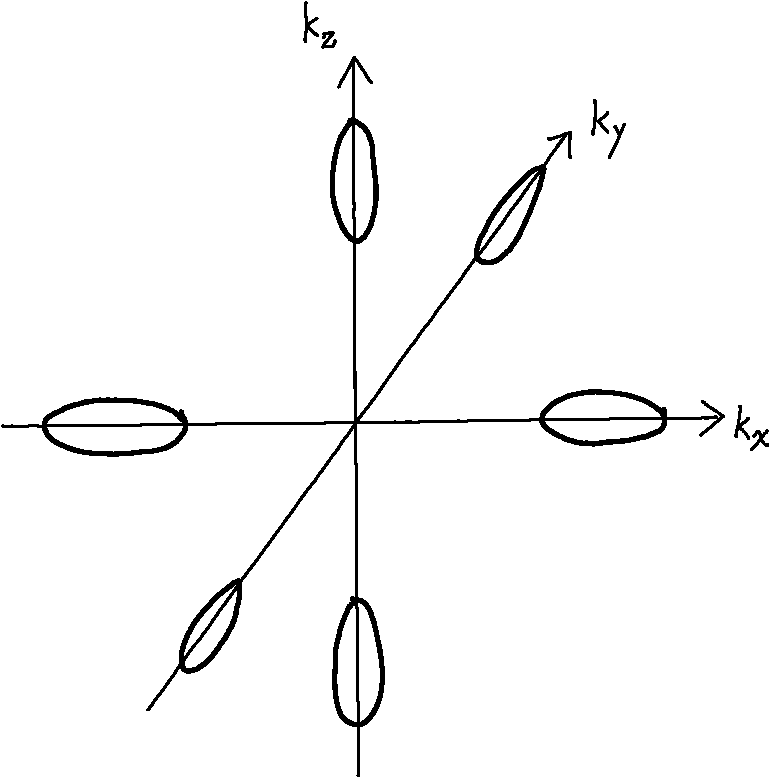
\includegraphics[width=.6\linewidth]{q3-equienergy}
	\end{figure}
	
	Volume of ellipsoid: $V = \diagfrac{4}{3} \pi k_x k_\perp^2$ where $k_\perp$ is the semi major axis length in the $y$, $z$ axes.
	
	Mass tensor suggests that (1/2 to account for spin degeneracy):
	\begin{align*}
		\frac{k_\perp^2}{0.2} &= k_x^2 \\
		\Rightarrow V &= \frac{4}{3} \cdot 0.2 \pi k_x^2 = \frac{1}{2}n \mtext{where $n$ is the density of charge carrier} \\
		\Rightarrow k_x &= \sbracket{\frac{1}{2}n \cdot \frac{3}{4} \cdot 5 \cdot \frac{1}{\pi}}^{1/3}
	\end{align*}
	
	Normal to (1 0 0), we have a circular cross section, and so $A_\textnormal{ext}$ is:
	\begin{align*}
		\pi k_\perp^2 &= 0.2\pi k_x^2 \\
		&= 0.2 \pi \sbracket{\frac{15}{8\pi}n}^{2/3}
	\end{align*}
	
	Thus we have the associated period $\Delta\rbracket{1/B}$:
	\begin{align*}
		\Delta\rbracket{\frac{1}{B}} &= \frac{2\pi e}{\hbar} \cdot \frac{1}{A_\textnormal{ext}} \\
		&= \frac{2\pi e}{\hbar} \cdot \frac{5}{\pi} \sbracket{\frac{8\pi}{15n}}^{2/3} \\
		&= \SI{0.46}{\per\tesla}
	\end{align*}
	
	And the corresponding frequency is $F = 1/\Delta(1/B) = \SI{2.17}{\tesla}$.
	
	Range: $0-\SI{10}{\tesla}$ since that is about the maximum B field generated by most laboratory equipments.
	
	Oscillation in resistivity should follow the above oscillation as $\rho \propto 1/J \propto 1/n$ so it is sensitive to the perturbation of Fermi surface:
	\begin{figure}[H]
		\centering
		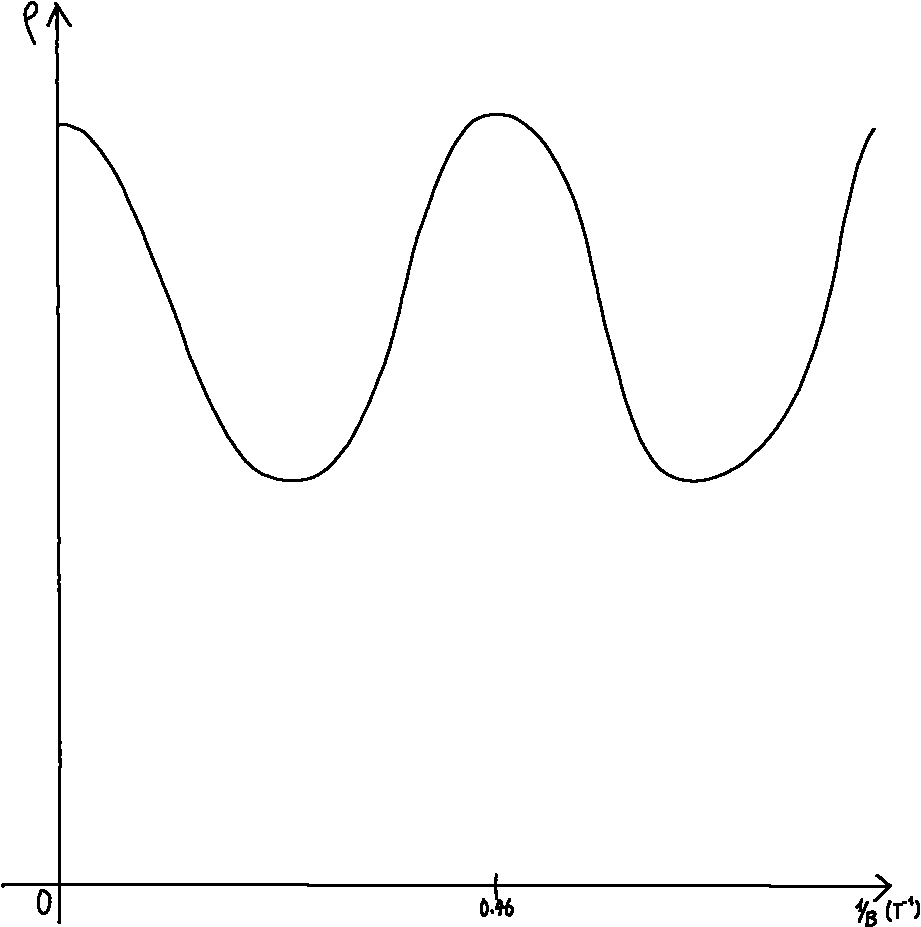
\includegraphics[width=.5\linewidth]{q3-rho}
	\end{figure}
	
	\part For Landau levels to be observable, $\omega\tau \gg 1$:
	\begin{align*}
		\Rightarrow \frac{eB}{m_y} &\gg \frac{1}{\tau} \\
		\Rightarrow T &\ll \SI{840}{\kelvin}
	\end{align*}
	
	Mobility $\mu = e\tau / m$:
	\begin{align*}
		\mu B &\gg 1 \\
		\Rightarrow \mu &\gg \SI{0.1}{\per\tesla}
	\end{align*}
	
	To verify the mass values, we may perform an angle-resolved photoelectron spectroscopy (ARPES) to obtain the band structure near Fermi level.
	Then we would have the mass tensor given by $M_{ij} = 1/\hbar \; \partial E/\partial k_i \; \partial k_j$.
\end{parts}